\documentclass[tikz]{standalone}
\begin{document}

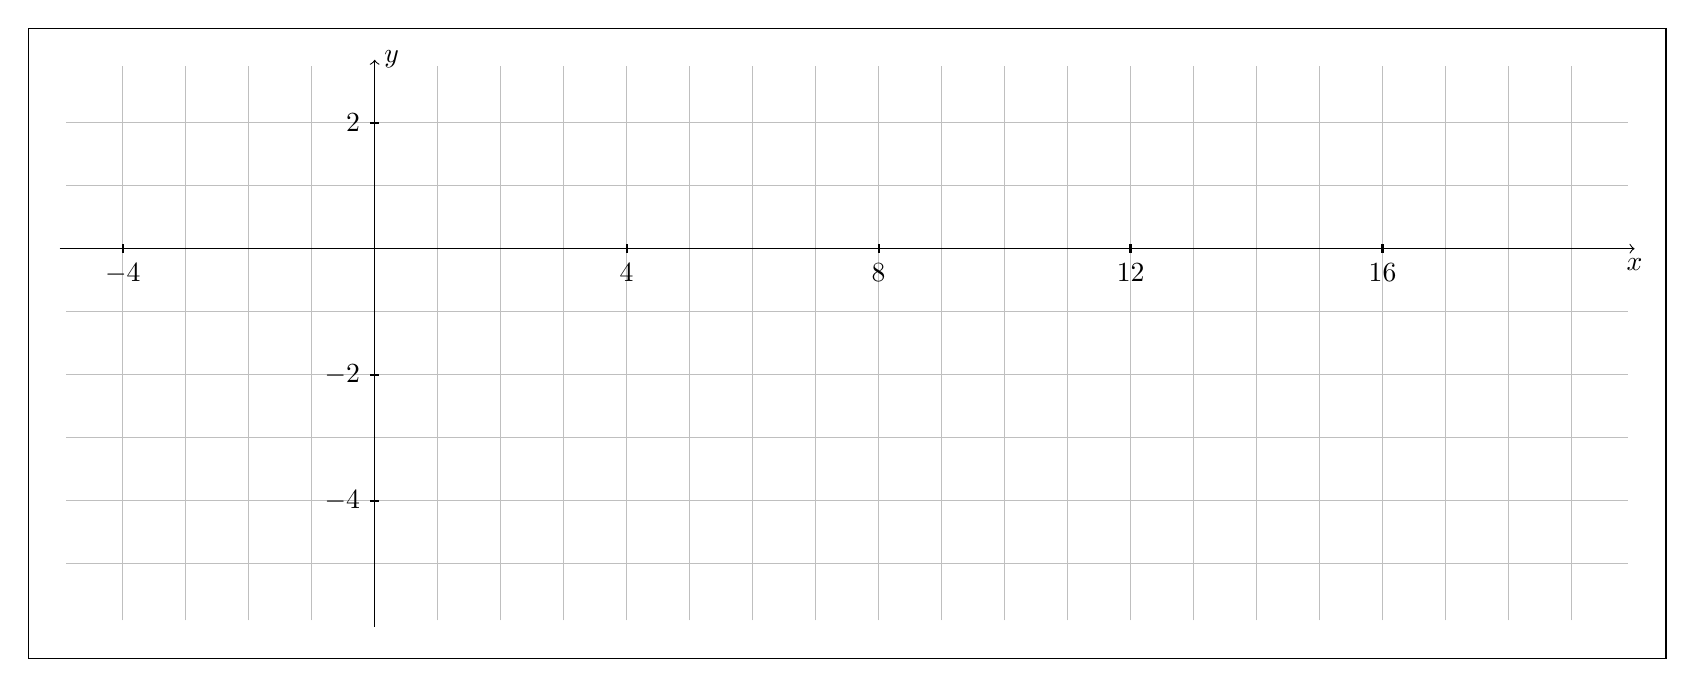
\begin{tikzpicture}[scale=0.8]

\draw[black,fill=white] (-5.5,-6.5) rectangle (20.5,3.5);
\draw[very thin,color=lightgray,step=1] (-4.9,-5.9) grid (19.9,2.9);

      \draw[->] (-5,0) -- (20,0) node[below] {$x$};
      \draw[->] (0,-6) -- (0,3) node[right] {$y$};
%\draw[domain=-5:20,smooth,variable=\x,black,ultra thick,samples=100] plot ({\x},\x/4 - 13/4);
       
      % tick marks
\foreach \x in {-4,4,8,12,16} 
	\draw [thick] (\x cm,2pt) -- (\x cm,-2pt) node[below] {$\x$};
\foreach \y in {-4,-2,2} 
	\draw [thick] (2pt,\y cm) -- (-2pt,\y cm) node[left] {$\y$};

    \end{tikzpicture}
\end{document}
